\section{3DGS Viewer: learning Gaussian splatting on the web}\label{sec:p3}

\subsection{Purpose}

3D Gaussian splatting \citep{kerbl2023} is a new way to capture real places and objects in 3D from ordinary photos or video, and it is quickly showing up in GIS and digital-twin tools. I wanted to understand what a splat actually is, how it can be shown in a web browser, and what a working implementation looks like. The result is a viewer where you open your own splat file and inspect it; the file is read in the browser and never uploaded.

\paragraph{A change of plan.} The first version was a CesiumJS globe with a gallery of georeferenced splats from around the world. It turned out that the example splats only loaded with a special evaluation token from Cesium, not with my own account, and another dataset depended on a share key that expires in December 2026. A public website cannot rely on that, so I rebuilt the project as a viewer for local files. The lesson was to check data access and licences \emph{before} building on a dataset.

\subsection{What I built}

\begin{itemize}
  \item Open a splat file by dialog or drag and drop (PLY, SPZ, \code{.splat}, \code{.ksplat} or SOG).
  \item A ``file facts'' panel that reads the file header: number of splats, size, colour detail and extent.
  \item An up-axis switch and a reset button, because splat files do not agree on which way is up.
  \item A two-point distance tool.
\end{itemize}

\subsection{What I learned about Gaussian splats}

\paragraph{What a splat is.} A splat scene is a cloud of hundreds of thousands of small, semi-transparent, coloured 3D blobs (Gaussians). Each has a position, a size and orientation, an opacity and a colour that changes with the viewing angle. Unlike a mesh, there are no surfaces; unlike a point cloud, each point has a shape. The blobs are optimised so that the scene \emph{looks} right from the photos, which is why splats look so realistic.

\paragraph{What is inside the file.} Reading the PLY header myself showed that most of each record is colour: of the 59 values stored per splat in a typical file, 45 describe how the colour changes with viewing direction. This explains why splat files are large and why compressed formats such as SPZ and SOG exist.

\paragraph{Splats and GIS.} Testing with real files showed what a splat does \emph{not} contain. It has no coordinate reference system, and it does not say which way is up: the files I tested were upright with $-Y$ as up, the usual convention for 3DGS training output, but lay on their side with $+Z$, the usual convention in GIS (\cref{fig:p3-upaxis}). It also has no real scale: measuring across the lid of a jar gave 1.075 ``units'', and nothing in the file says what a unit is. To use splats in GIS, they must be georeferenced, for example with GNSS or ground control points, and can then be streamed onto a globe as 3D Tiles \citep{3dtiles,khr-gaussian-splatting}, which is what my first version tried to do.

\begin{figure}[htbp]
\centering
\begin{subfigure}{0.49\textwidth}
  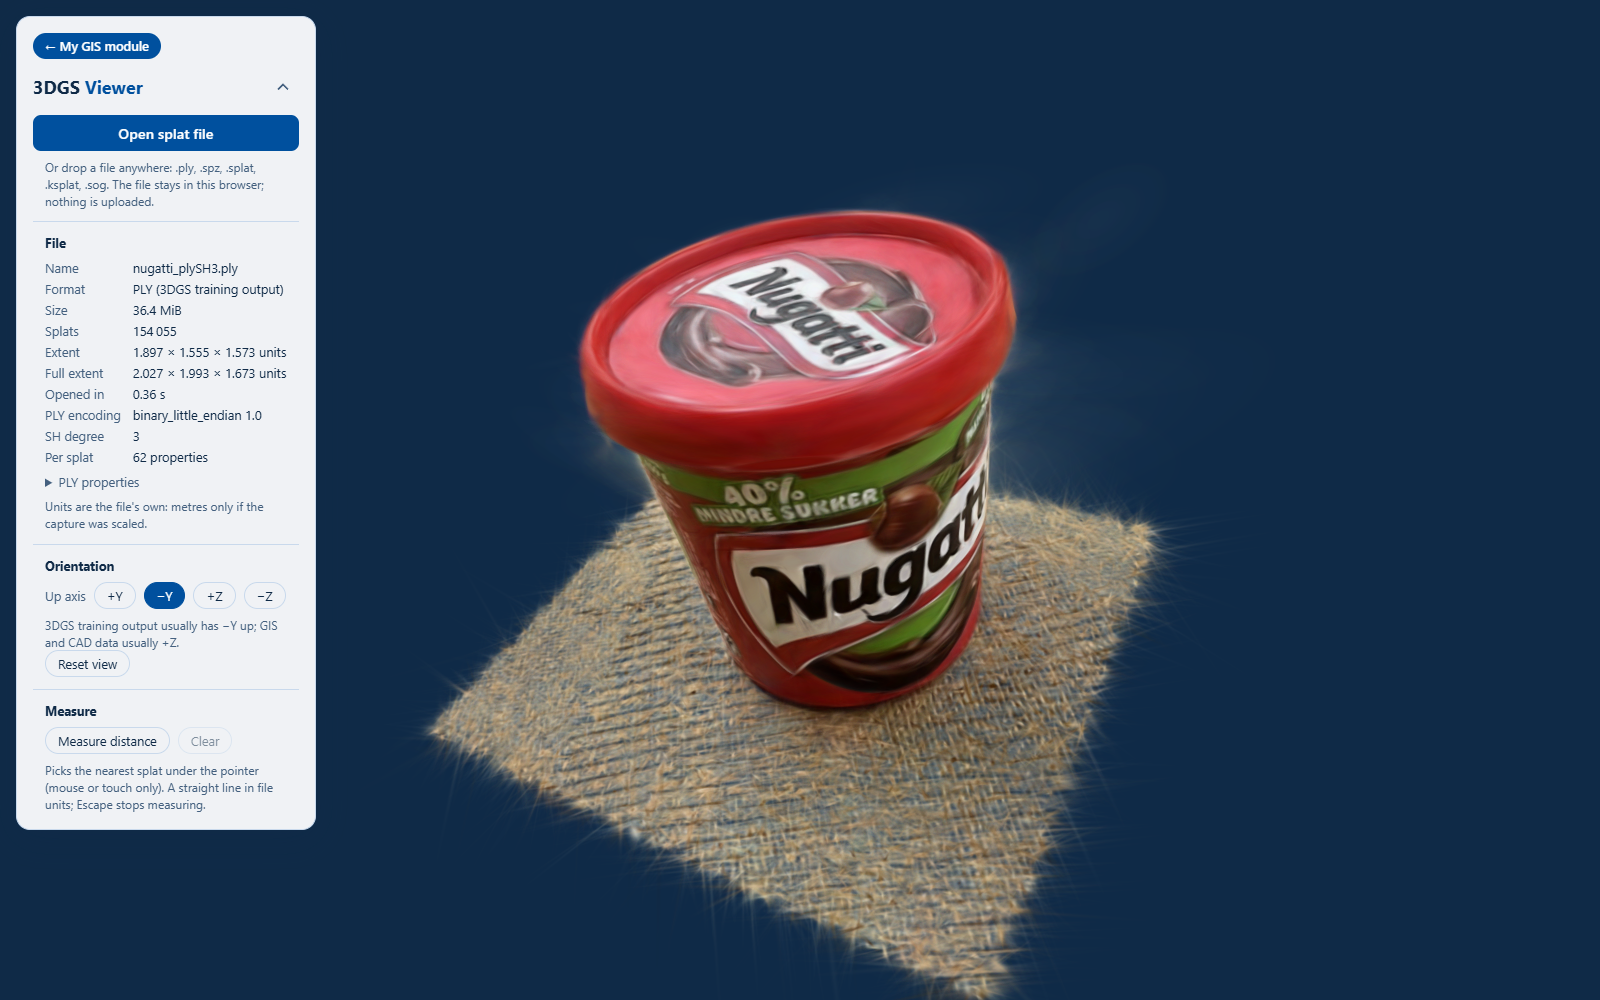
\includegraphics[width=\linewidth]{project-3-02-loaded-file-facts.png}
  \caption{Up axis $-Y$: upright}
\end{subfigure}\hfill
\begin{subfigure}{0.49\textwidth}
  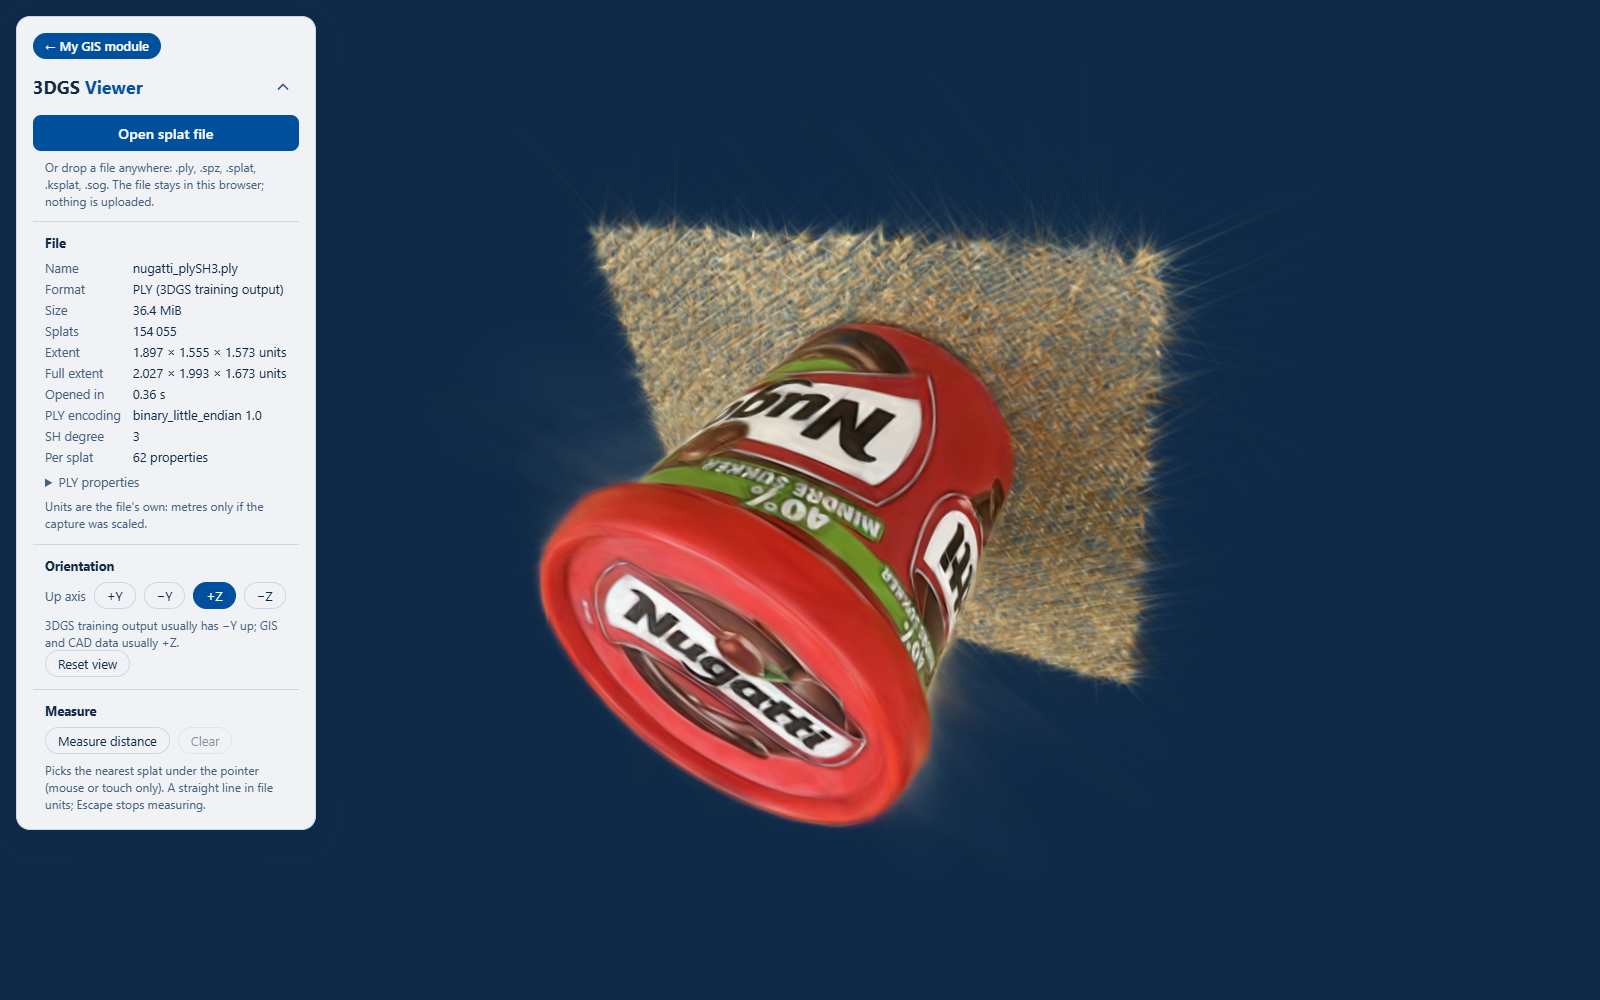
\includegraphics[width=\linewidth]{project-3-03-up-axis-wrong-plus-z.png}
  \caption{Up axis $+Z$: on its side}
\end{subfigure}
\caption{A splat of a Nugatti jar in the viewer, with the file facts in the panel. The file does not say which way is up, so the same data appears upright or on its side depending on the convention. Rendering: Spark and three.js (MIT).}
\label{fig:p3-upaxis}
\end{figure}

\subsection{What I learned about the web technology}

The viewer uses Spark \citep{spark}, a splat renderer built on three.js \citep{threejs}, the most common 3D library for the web. I learned how a three.js scene is organised (renderer, scene, camera and controls), how picking works by casting a ray from the mouse into the scene, and why the splats must be sorted by depth every time the view changes. Reading files locally, with no server or upload, keeps the app simple and private, but the renderer makes the download large before anything can be shown. Stray blobs far from the scene (``floaters'') are common in captures, so the camera is framed on the central part of the scene rather than on all splats.
